\section{Ultramarinblau}
\authors{Sophia Ivaschuk, Gala Gottschalg}

Ultramarinblau ist ein 5000 Jahre altes, anorganisches Farbpigment. Es ist ein Mineral, welches in den Farben Blau, Violett, Pink und Grün vorkommt. Wegen seiner Seltenheit war es früher teurer als Gold. Heute werden pro Jahr 20000 t synthetisch hergestelltes Ultramarinblau verwendet.
Besonders beliebt und geeignet für vielfältige Anwendungen ist Ultramarin durch seine chemischen beziehungsweise physikalischen Eigenschaften. Je nach Pigment ist es bei Temperaturen bis zu 400$^{\circ}C$ und einem pH-Wert zwischen 6 und 9 stabil. Zusätzlich besitzt das geruchlose Ultramarin eine hohe Lichtechtheit, das heißt, die Farbe verblasst auch bei intensiver Bestrahlung nicht. Durch  seine hohe Oberflächenenergie ist der Farbstoff kohäsiv. Er ist nicht mutagen. Somit geht kein Gefahrenpotential von ihm aus, sodass Ultramarin sogar in Kinderspielzeug und Kosmetika verwendet wird. Außerdem findet man ihn  in Seifen und Waschmitteln. 
Früher wurde Ultramarin vor allem in der Kunst verwendet. Besonders beliebt war es bei Malern wegen seiner Lichtechtheit. So verwendeten auch schon die alten Ägypter die Farbe in Totenmasken, bei der Bemalung von Tierfiguren und in Mosaiken.

Um die chemischen und physikalischen Eigenschaften zu verstehen, muss die chemische Struktur des Ultramarins näher beleuchtet werden.
Es besteht aus einem Sodalithkäfig, in welchem die Polysulfidanionen $S_2^{-}$, $S_3^{-}$ und $S_4^{-}$ eingeschlossen sind [Abb.\ref{fig:Ultramarin}].
Der Sodalithkäfig ist ein dreidimensionales Aluminiumsilikatgitter. Dieses besteht aus $SiO_{4}^{-}$- und $AlO_{4}^{-}$-Tetraedern mit zusätzlichen Natrium- und Chloridionen. Die Verhältnisformel des Kristallgitters ist somit $[Na_{8}Al_{6}Si_{6}O_{24}]^{2+}$.
Verantwortlich für die Farbigkeit sind die eingeschlossenen Polysulfidanionen. Diese absorbieren Licht unterschiedlicher Wellenlängen. Je nach dem, wie viele und welche Polysulfidanionen vorliegen, variiert die Farbe. So kommt es zu den unterschiedlichen Farben der Pigmente. 

\begin{dsafigure}
 \centering
 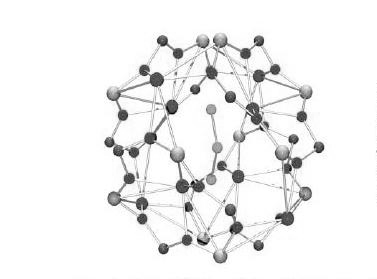
\includegraphics[width=\columnwidth]{Sodalithkaefig.png}
 \caption{Struktur des Ultramarins. \cite{sideplayer}}
 \label{fig:Ultramarin}
\end{dsafigure}

Lange Zeit konnte Ultramarin nicht synthetisch hergestellt werden. Die Gewinnung aus den Lagerstätten in Chile und Afghanistan war bei geringer Ausbeute sehr zeitintensiv und aufwändig. Erst 1826 gelang Guimet die Synthese des ersten künstlichen Ultramarins. 1834 wurde die erste Fabrik eröffnet. Zur Herstellung werden Porzellanerde, Feldspat, wasserfreies Natriumcarbonat, Schwefel und ein reduzierendes Mittel verwendet. Zunächst wird die Porzellanerde bei 700$^{\circ}C$ aktiviert. Die Mischung findet danach bei 750$^{\circ}C$ statt. Dabei reagiert das Natriumcarbonat mit Schwefel und dem reduzierenden Mittel zu Natriumpolysulfid, eingelagert in die sodalithische Struktur. Damit ist die Produktion heute relativ kostengünstig und mit einer Ausbeute von 75\% blauem Ultramarin im Rohprodukt recht ertragreich. 
\cite{Buxbaum} 
\cite{Seel}
